% Measuring the RudriQ Linker: arXiv-ready preprint.
% Compile: pdflatex paper && bibtex paper && pdflatex paper && pdflatex paper
% (Overleaf: upload paper.tex + refs.bib + figs/ and recompile.)
% arXiv author metadata: given name = "Kishan Raj", family name = "VG".
\documentclass[11pt]{article}

\usepackage[T1]{fontenc}
\usepackage[utf8]{inputenc}
\IfFileExists{lmodern.sty}{\usepackage{lmodern}}{}  % optional: nicer fonts if available
\usepackage[margin=1in]{geometry}
\usepackage{graphicx}
\usepackage{amsmath,amssymb}
\usepackage{booktabs}
\usepackage{array}
\usepackage[protrusion=true,expansion=false]{microtype}  % expansion=false: works without scalable fonts
\usepackage{enumitem}
\usepackage{authblk}
\usepackage{xcolor}
\usepackage[numbers,sort&compress]{natbib}
\usepackage[hidelinks]{hyperref}
\hypersetup{pdftitle={Measuring the RudriQ Linker: Accuracy, Calibration, and a Trust Envelope for Cross-Domain Data-to-LLM Provenance},pdfauthor={Kishan Raj VG}}

% Convenience macros for the recurring special characters.
\newcommand{\dto}{\ensuremath{\rightarrow}}     % data->LLM arrow
\newcommand{\us}{\ensuremath{\mu}\textrm{s}}    % microseconds

% Let TeX stretch interword spacing on stubborn lines (long \texttt tokens,
% hyphenated bold compounds) rather than running into the margin.
\setlength{\emergencystretch}{3em}

\title{Measuring the RudriQ Linker: Accuracy, Calibration, and a\\
Trust Envelope for Cross-Domain Data\dto{}LLM Provenance}

\author{Kishan Raj VG\thanks{Full legal name: Kishan Raj Vandhavasi Goutham Kumar.
The author publishes as ``Kishan Raj VG.''}}
\affil{University of the Cumberlands, PhD Program, Graduate Information Technology,
Williamsburg, Kentucky, USA\\ \texttt{kishanraj41@gmail.com}}
\date{August 2026}

\begin{document}
\maketitle

\begin{abstract}
Modern ML systems increasingly cross a domain boundary that existing observability tools do not: data
prepared by pandas/Spark flows into LLM calls (embeddings, chat completions). \emph{The RudriQ linker}
attempts to recover this \textbf{data\dto{}LLM lineage} automatically, attaching a confidence-scored
provenance edge from an upstream data artifact to each LLM call. The central question for an audit tool is
not whether such a linker \emph{exists} but whether its links are \emph{correct}, and that has gone
unmeasured, because cross-domain ground truth is hard to establish.

We contribute a \textbf{construction-based benchmark} that makes ground truth tractable: pipelines in which
we assign every node identity, so the true data\dto{}LLM edge set is known \emph{by construction}, paired
with an adversarial arm built to make the linker fail. \textbf{All findings below are established on this
synthetic and adversarial corpus; ecological validation on real third-party pipelines is in progress}, and
we mark throughout which quantities are portable linker properties and which are corpus-composition-dependent.

On the constructed corpus we find: \textbf{(1)} the linker's per-link confidence scale is \textbf{calibrated
in structure}: measured precision falls monotonically as stated confidence falls, a \emph{structural}
property (as distinct from the specific per-band precision \emph{values}, which are composition-dependent);
this is the keystone result. \textbf{(2)} the exact-match strategy (object-identity) is near-perfectly
precise (precision 1.000, 95\% CI [0.987, 1.000], $n=300$), and \textbf{no false positives were observed on
representative new data} (0 of 200; 95\% CI upper bound below 2\%). \textbf{(3)} the false-positive surface
comprises \textbf{two bounded, characterized mechanisms} that respect their boundaries, yielding a
confidence-threshold \emph{deployment guideline}. \textbf{(4)} common-path instrumentation overhead is
\textbf{below 0.1\% of a single LLM call}, with two characterized and mitigable fallback costs.

This is \textbf{Paper~2} of the RudriQ/AutoLineage line. \textbf{AutoLineage (Paper~1)}~\cite{vg2026autolineage}
contributes the import-time \emph{capture mechanism}; \textbf{this paper measures the cross-domain
\emph{linker's accuracy and calibration}.} Same system, different contribution.
\end{abstract}

\section{Introduction}

Data lineage and ML observability tools trace operations \emph{within} a domain (DataFrame
transformations, training steps, or, separately, LLM call traces) but not \emph{across} the boundary
where prepared data enters a language model. In a retrieval-augmented generation (RAG) or ML+LLM pipeline,
the provenance question a practitioner and an auditor both ask is: \emph{which upstream data artifact
produced the input to this LLM call?} Answering it requires linking a data-domain node to an LLM-domain
node, a \textbf{cross-domain lineage link} that no general-purpose lineage system recovers automatically
\cite{openlineage,zaharia2018mlflow,openllmetry}.

The RudriQ linker recovers these links at import time, with no user annotation, by maintaining process-local
registries of tracked objects and correlating each LLM call's input against them. It applies an
\emph{ordered} set of matching strategies and attaches a fixed per-strategy confidence to each emitted edge.

The problem is \textbf{measurement}, not mechanism. A mechanism paper is accepted if the idea is novel and
works; an empirical paper is accepted only if the \emph{evaluation methodology is sound}. For a cross-domain
linker, soundness turns on a single hard question: \textbf{what is ground truth, and how do you establish
it?} ``Correct'' is exactly the thing that is difficult to pin down for cross-domain lineage, and a flawed
ground-truth definition invalidates every downstream number.

Our contributions:
\begin{enumerate}[leftmargin=*]
\item A \textbf{construction-based benchmark methodology} in which ground truth is known \emph{by
construction} (we assign node identities and choose which data feeds which LLM call), with a deliberately
\textbf{adversarial negative arm} that exists to make the linker fail and to supply the false-positive-rate
denominator.
\item A \textbf{scoring harness} that scores production (first-match-wins) and per-strategy \emph{shadow}
outcomes against ground truth, computing precision, recall, FPR, and \textbf{confidence calibration} with
Wilson intervals, and that \emph{structurally enforces} the honesty distinctions an empirical reviewer
checks.
\item Four empirical findings (calibration, per-strategy accuracy, a characterized FP surface, overhead),
each reported with its uncertainty and an explicit portable-vs-composition-dependent split.
\item A \textbf{trust-envelope map}: the failure surface connected to the calibration result as an
actionable confidence-threshold deployment guideline.
\end{enumerate}

\section{Related Work}

\paragraph{Data lineage / provenance.} Open standards and platforms such as OpenLineage~\cite{openlineage}
and DataHub~\cite{datahub} capture lineage \emph{within the data domain}: datasets, jobs, and
column-level edges (DataHub derives the latter by SQL parsing), on foundations formalized by Cheney et
al.~\cite{cheney2009provenance}. These establish lineage \emph{graphs}, and some even \emph{infer} edges,
but they remain inside the data domain and report lineage as a catalog feature; none crosses the
data\dto{}LLM boundary or \emph{measures} an inferred linker's accuracy and calibration against constructed
ground truth with adversarial negatives.

\paragraph{ML experiment + pipeline tracking.} MLflow~\cite{zaharia2018mlflow} and Weights \&
Biases~\cite{wandb} capture runs, parameters, metrics, and artifacts via \textbf{explicit instrumentation}; lineage is recorded when the developer logs it. AutoLineage~\cite{vg2026autolineage} (Paper~1) removes
the instrumentation via import-time hooking, but, like the above, is a \emph{capture} contribution. None
evaluates a cross-domain linker's accuracy; capture and measured-inference are different contributions.

\paragraph{LLM observability / tracing.} OpenLLMetry/Traceloop~\cite{openllmetry},
LangSmith~\cite{langsmith}, Langfuse~\cite{langfuse}, and Arize Phoenix~\cite{phoenix} trace LLM calls (model, tokens, latency, prompt/completion), typically over OpenTelemetry. They treat the \emph{data that
produced the prompt} as out of scope; the data\dto{}LLM edge our linker recovers is precisely the gap these
tools leave.

\paragraph{RAG / retrieval evaluation.} RAGAS~\cite{es2024ragas}, ARES~\cite{saadfalcon2024ares}, and
TruLens~\cite{trulens} evaluate \emph{answer and retrieval quality}: faithfulness, groundedness,
context/answer relevance. This is an \textbf{orthogonal axis} to \emph{provenance-link correctness}: they
ask whether the answer is well-grounded, not whether a recovered data\dto{}LLM lineage edge is the right
edge.

\paragraph{Confidence calibration.} Reliability diagrams and empirical calibration evaluation are
established~\cite{niculescu2005probabilities,guo2017calibration}. We apply the same diagnostics (precision conditioned on stated confidence, monotonicity, Wilson intervals) to a \emph{rule-based} linker
whose confidence is \textbf{assigned per strategy} rather than learned, which makes calibration a falsifiable
claim about a fixed five-value scale.

\paragraph{Closest prior work, and the boundary of our novelty.} Two recent works sit nearest. Yin et
al.~\cite{yin2025schemalineage} benchmark language models on extracting \emph{schema lineage} from
multilingual pipeline scripts, scoring with their Schema Lineage Composite Evaluation (SLiCE) metric, which combines structural correctness with semantic fidelity, over four components (source schemas, source tables,
transformation logic, aggregation operations). It shares our \emph{measure-the-extraction} stance but
differs on the two axes that define our contribution: it stays \textbf{within the data domain}
(schema-to-schema lineage in code, not data\dto{}LLM-call edges), and it benchmarks \textbf{LLMs as
extractors}, not a \emph{rule-based} linker's precision/recall and \textbf{confidence calibration} under
adversarial negatives. Zhao~\cite{zhao2025xprov} (XProv), a vision paper, proposes a common parameterized
representation for \textbf{cross-library} lineage in data-science workflows, linking materialized lineage
graphs to abstracted logical patterns; it is the closest work on \emph{crossing boundaries}, but the
boundary it crosses is library-to-library \emph{within} the data domain, it is architectural rather than an
evaluated system, and it neither links to LLM calls nor measures accuracy. We therefore do \textbf{not}
claim that lineage extraction is unmeasured (it is, in-domain~\cite{yin2025schemalineage}) nor that
cross-boundary lineage is unconsidered (it is, across libraries~\cite{zhao2025xprov}). We claim novelty for
a specific, and to our knowledge unoccupied, combination: crossing the \textbf{data\dto{}LLM-call} boundary,
with a \textbf{rule-based linker} whose edges are \textbf{measured for accuracy and calibration} against a
\textbf{construction-based benchmark with adversarial negatives}.

\section{The Linker Under Test}

The linker's public entry point is \texttt{correlate(llm\_input, span\_attributes)} \dto{} \texttt{(parent\_id,
method, confidence)}. It applies an \textbf{ordered} tuple of strategies and returns the \textbf{first}
non-\texttt{None} match (\emph{first-match-wins}). The strategies and their \textbf{fixed} confidences:

\begin{table}[h]
\centering
\small
\begin{tabular}{@{}cl l p{7.2cm}@{}}
\toprule
Order & Strategy & Confidence & Mechanism \\
\midrule
1 & \texttt{object\_identity} & 1.0 / 0.95 & Python \texttt{id()} match against the in-process object
registry (1.0 for the input itself; 0.95 for a registered element of a list/tuple input). \\
2 & \texttt{content\_hash} & 0.8 & SHA-256 of the whole input against persisted node hashes
(storage-backed). \\
3 & \texttt{substring} & 0.7 / 0.5 & Full-containment match (length-floored at 20 chars) between input
strings and registered upstream strings. \\
4 & \texttt{name\_match} & 0.5 & Heuristic by variable/column name; \textbf{a stub returning
\texttt{None}} in the evaluated version. \\
\bottomrule
\end{tabular}
\end{table}

Two properties drive the evaluation. \textbf{First, confidence is assigned per strategy/branch, never
learned}: there are exactly five discrete values $\{1.0, 0.95, 0.8, 0.7, 0.5\}$, which makes
precision-conditioned-on-confidence a \emph{falsifiable} calibration claim. \textbf{Second, first-match-wins
makes cost and behavior bimodal}: a high-precedence strategy can pre-empt a lower one, and the expensive
strategies run only on a miss of the cheap one (\S5.5, \S5.6).

\section{Methodology}

\subsection{The trichotomy (the crux)}

Every candidate LLM call is labeled into one of three ground-truth classes, because \textbf{a non-link is
not always an error}:
\begin{itemize}[leftmargin=*]
\item \textbf{LINKED-TRUE}: the input derives from a specific registered upstream node; the linker
\emph{should} emit the correct link. Contributes to recall.
\item \textbf{TRUE-NEGATIVE}: the input is genuinely new data with no in-scope provenance (e.g.\ a fresh
user query); the linker \emph{should} stay silent. A fire here is a false positive; this pool is the FPR
denominator.
\item \textbf{OUT-OF-SCOPE}: provenance exists but outside what the linker can observe; excluded from
recall \emph{and} from the FPR pool, reported only as a coverage gap.
\end{itemize}
Recall is computed over LINKED-TRUE only; FPR over TRUE-NEGATIVE only. Conflating ``should link and didn't''
with ``correctly didn't link'' would make recall arbitrary; this is the single most important methodological
decision in the benchmark.

\subsection{Three arms}
\begin{itemize}[leftmargin=*]
\item \textbf{Arm A (synthetic, control).} Pipelines where we assign every \texttt{node\_id}, so the true
edge set is known by construction. Each LINKED-TRUE link is tagged with the \textbf{mechanism class} it
should be caught by: \emph{verbatim-object, element-of-collection, exact-copy, templated-containment,
paraphrased-derived}, plus deliberate \textbf{strategy-collision} pipelines (one input satisfying two
strategies at \emph{different} true parents) to make pre-emption measurable.
\item \textbf{Arm C (adversarial, negative).} Built to make the linker fail and to supply the TRUE-NEGATIVE
pool: clean true-negatives, near-misses just below threshold, generic-content substring collisions, and
content-hash aliasing traps.
\item \textbf{Arm B (real, ecological).} Annotated third-party pipelines, with inter-annotator agreement
($\kappa$). \textbf{In progress}; supplies the representative input distribution and the pre-emption
\emph{correctness} evidence (\S5.5, \S6).
\end{itemize}

\subsection{Registered-vs-inferred and the self-proving gate}

For object-identity links the upstream object \emph{is} registered (the control). For inferred strategies
(content-hash, substring) the dataflow genuinely exists but the matching object is \textbf{not}
identity-registered; the linker must infer it. A per-pipeline \textbf{construction-consistency gate} runs
each pipeline through the real linker and asserts the \emph{fired} strategy matches the \emph{constructed}
mechanism class (a substring pipeline where object-identity fired is a corpus bug, hard-failed at
generation). Assembly \textbf{refuses to emit a corpus containing a failing gate}, so a shipped corpus
provably tests what it claims.

\subsection{Determinism and pre-registration}

Corpora are seeded and serialize \textbf{byte-identically} across runs (verified by diff); LLM HTTP is
mocked, so the linker always sees the real Python object.

\paragraph{Pre-registered vs.\ implementation-resolved (stated plainly, because the distinction is the
point).} We pre-registered the methodology before any corpus existed: the trichotomy and its scoring roles,
the three-arm design, the $\kappa$ protocol, the symmetric-collision decision, and the mechanism-class
tagging. Implementation then \textbf{forced refinements we did not foresee}, recorded in full and dated in
the methodology log and explicitly \textbf{not} backdated into the pre-registration. Three reshape how
results are \emph{scored}: \textbf{(S1)} a wrong-parent link is simultaneously a precision-error, a
recall-miss, and \emph{not} a false-positive-rate event, so precision/recall/FPR are computed over three
different populations; \textbf{(S2)} the FPR denominator is the \emph{representative} clean true-negative
pool, with adversarial decoys reported separately (\S5.3--5.4); \textbf{(S3)} blended precision/FPR are
corpus-composition-dependent and so are not headline numbers. A fourth, surfaced only at scale-up, bounds
what may be \emph{quoted}: tightening an interval does not make a composition-dependent value a linker
property, so we report the monotonic \emph{structure} and the composition-robust quantities as findings
while treating per-band \emph{values} as on-corpus. (The OUT-OF-SCOPE pooling rule of \S4.1 is likewise an
implementation-resolved clarification.) We state this split in the paper rather than only in the log,
because presenting implementation-forced decisions as foresight would claim a rigor we did not have; the
honest admission is the credibility gain.

\section{Results}

Unless noted, figures are from the harness at scale (Arm A: $n=100$ per mechanism class; Arm C: 200 clean
true-negatives, 25 per decoy kind; 900 calls total), run against the real linker. Accuracy figures are
deterministic. Intervals are Wilson 95\%. \textbf{All results below characterize the linker \emph{on the
constructed corpus}; we do not claim they generalize to arbitrary real workloads until ecological validation
lands (\S8). Every headline figure should be read with that ``on the constructed corpus'' tether attached.}

\subsection{Calibration (the keystone)}

Precision conditioned on stated confidence is \textbf{monotonic} (precision does not increase as confidence falls) at $N=900$:

\begin{table}[h]
\centering
\small
\begin{tabular}{@{}lllcl@{}}
\toprule
Stated confidence & Measured precision & 95\% CI & $n$ & Carried by \\
\midrule
1.00 & 1.000 & [0.963, 1.000] & 100 & \texttt{object\_identity} (verbatim) \\
0.95 & 1.000 & [0.981, 1.000] & 200 & \texttt{object\_identity} (element) + collision \\
0.80 & 0.800 & [0.721, 0.861] & 125 & \texttt{content\_hash} (exact-copy + aliasing) \\
0.70 & 0.800 & [0.721, 0.861] & 125 & \texttt{substring} (templated + collision) \\
\bottomrule
\end{tabular}
\end{table}

\begin{figure}[h]
\centering
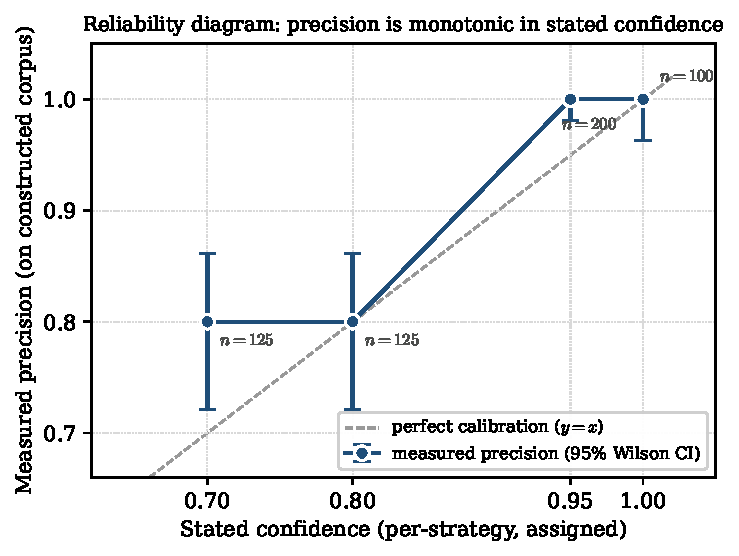
\includegraphics[width=0.72\linewidth]{figs/reliability.pdf}
\caption{Reliability diagram for the linker's five-value confidence scale (on the constructed
corpus, $N=900$). Measured precision does not increase as stated confidence falls: the \emph{monotonic structure} that is the keystone calibration finding. Error bars are 95\% Wilson
intervals; the high bands ($1.0/0.95$) show no observed errors, and the false-positive surface lands in
the lower bands. The per-band \emph{values} (notably $0.800$) are corpus-composition-dependent and are
not quoted as bare linker properties; the \emph{monotonicity} is.}
\label{fig:reliability}
\end{figure}

On the constructed corpus, the confidence scale is \textbf{calibrated in structure}: the high bands show no
observed errors (precision 1.000, lower bound $>0.96$); the false-positive surface lands precisely in the
lower bands where the riskier inferred strategies live. This is the assertion\dto{}measured-result
transformation the paper sets out to demonstrate.

\paragraph{Honesty boundary (portable vs.\ composition-dependent).} The \emph{monotonic structure} (precision not increasing as confidence falls) is what we report as the calibration finding; the
\emph{values} of the lower bands (0.800) are \textbf{corpus-composition-dependent} (0.800 is exactly the
100:25 true-positive : adversarial-decoy ratio chosen for the corpus) and would become real linker
properties only against a representative input distribution. We observed the structure on this corpus at
$N=900$; we did not run a composition sweep, so we claim the structure as a \emph{reported finding}, not as
composition-invariant. We therefore do not quote 0.800 as a bare linker property; we quote the
\emph{monotonicity}.

\subsection{Per-strategy accuracy (composition-robust)}

\begin{table}[h]
\centering
\small
\begin{tabular}{@{}llc@{}}
\toprule
Strategy & Precision (95\% CI) & $n$ \\
\midrule
\texttt{object\_identity} & \textbf{1.000} [0.987, 1.000] & 300 \\
\texttt{content\_hash} & 0.800 [0.72, 0.86] & 125 \\
\texttt{substring} & 0.800 [0.72, 0.86] & 125 \\
\bottomrule
\end{tabular}
\end{table}

\texttt{object\_identity} precision ($>0.98$, lower bound) is \textbf{composition-robust}: identity matching
is exact, so it produced no observed false positives across the clean/adversarial mix tested. The
content-hash and substring precision \emph{values} inherit the \S5.1 composition caveat.

\emph{Per-mechanism recall} (strategy-appropriate; conditional on the mechanism class, hence
composition-robust), $N=900$:

\begin{table}[h]
\centering
\small
\begin{tabular}{@{}llc@{}}
\toprule
Mechanism class & Recall (95\% CI) & $n$ \\
\midrule
verbatim\_object & 1.000 [0.963, 1.000] & 100 \\
element\_of\_collection & 1.000 [0.963, 1.000] & 100 \\
exact\_copy & 1.000 [0.963, 1.000] & 100 \\
templated\_containment & 1.000 [0.963, 1.000] & 100 \\
strategy\_collision & 1.000 [0.963, 1.000] & 100 \\
\textbf{paraphrased\_derived} & \textbf{0.000} [0.000, 0.037] & 100 \\
\bottomrule
\end{tabular}
\end{table}

The catchable mechanism classes are recovered with lower-bound recall $>0.96$. \textbf{Paraphrased-derived
is a recall ceiling, not a misfire} (\S8).

\subsection{False-positive rate (representative denominator)}

On the constructed corpus, over the \textbf{representative clean true-negative pool} ($n=200$): \textbf{FPR
$=$ 0.000, 95\% CI [0.000, 0.019]}: \textbf{no false positives were observed} on genuinely-new data (0 of
200), with a quotable upper bound below 2\%. The adversarial decoys are deliberately \textbf{excluded} from
this denominator (\S5.4): folding hard-by-construction decoys into FPR would inflate the headline rate, the
precise overclaim our methodology forbids. Two distinct notions of false positive are kept separate: a
\emph{precision-FP} (any incorrect emitted link, including a wrong-parent link on a positive) versus an
\emph{FPR-FP} (a link on a true-negative). A wrong-parent link is a precision-FP and a recall-miss but is
\textbf{not} in the FPR pool.

\subsection{The false-positive surface (Arm C)}

Arm C is designed to make the linker fail. It surfaces \textbf{two bounded, characterized mechanisms}:
\begin{itemize}[leftmargin=*]
\item \textbf{content-hash aliasing} (confidence 0.8, \emph{wrong-parent}): two upstream nodes with
identical content; the linker returns the most-recent, mis-attributing provenance.
\item \textbf{substring generic-collision} (confidence 0.7, \emph{spurious-link}): a generic
$\geq$20-char phrase incidentally fully contained in an unrelated prompt links the call to that phrase.
\end{itemize}
Critically, the \textbf{near-misses stayed silent}: an 18-char below-floor substring and a one-character-off
hash both produced no link. The linker's boundaries (the 20-char floor, exact-hash matching) \textbf{hold};
it fails \emph{only} where it is genuinely vulnerable. A bounded, explained failure surface is a stronger
result than reported perfection, which would read as a rigged adversarial arm.

\subsection{Pre-emption: two claims, separate evidence}

First-match-wins means a high-precedence strategy can mask a lower one. We report this as \textbf{two
distinct claims with two distinct evidence bases, never fused}:

\begin{quote}
\textbf{Claim 1: behavioral masking (measured, Arm A, high-$N$).} In strategy-collision pipelines,
production masks the substring-parent in favor of the object-identity parent at a rate of \textbf{1.000}
(95\% CI [0.963, 1.000], $n=100$ collisions at $N=900$). This is a \emph{behavioral} statement (\emph{what gets masked}) and carries no claim about which parent is ``more correct.''
\end{quote}

\begin{quote}
\textbf{Claim 2: correctness cost (deferred, Arm B, no synthetic evidence by design).} Whether
pre-emption ever masks the \emph{better} link is a correctness judgment that synthetic construction cannot
honestly make (in our symmetric collisions both edges are genuinely true). The harness's sharpest check, cases where production scored \emph{wrong} while a shadow strategy would have scored \emph{right}, returns
\textbf{0} at $N=900$, empirically confirming the symmetric construction produced symmetric outcomes. The
correctness claim therefore has \textbf{zero synthetic evidence by design} and awaits annotated real
pipelines.
\end{quote}

We deliberately keep these in separate paragraphs: fusing them into ``pre-emption causes errors'' would
inherit Claim~2's (absent) evidence onto Claim~1's broad behavioral result.

\subsection{Overhead (distributional; the bimodal insight)}

Overhead is the only \emph{non-deterministic} measurement; we report it distributionally (warmup discarded,
median + tail, noise floor measured at ${\sim}300$\,ns, GC disabled). \textbf{Environment-specific} (Win11,
Python 3.12.4, 8-core Intel); the \textbf{portable findings are the ratios and scaling shapes}, not the
absolute \us.

\begin{table}[h]
\centering
\small
\begin{tabular}{@{}lp{6cm}ll@{}}
\toprule
Strategy & Scaling shape ($10 \rightarrow 10^4$ entries) & Median @1k & p99 @1k \\
\midrule
\texttt{object\_identity} & \textbf{flat $O(1)$} & 3.2\us & 19.7\us \\
\texttt{content\_hash} & flat, but \textbf{$\approx$1000$\times$ identity} (storage I/O) & 3.50\,ms & 6.37\,ms \\
\texttt{substring} & \textbf{$O(n)$}: 11\us $\rightarrow$ 13.75\,ms & 1.15\,ms & 2.15\,ms \\
\bottomrule
\end{tabular}
\end{table}

\begin{figure}[h]
\centering
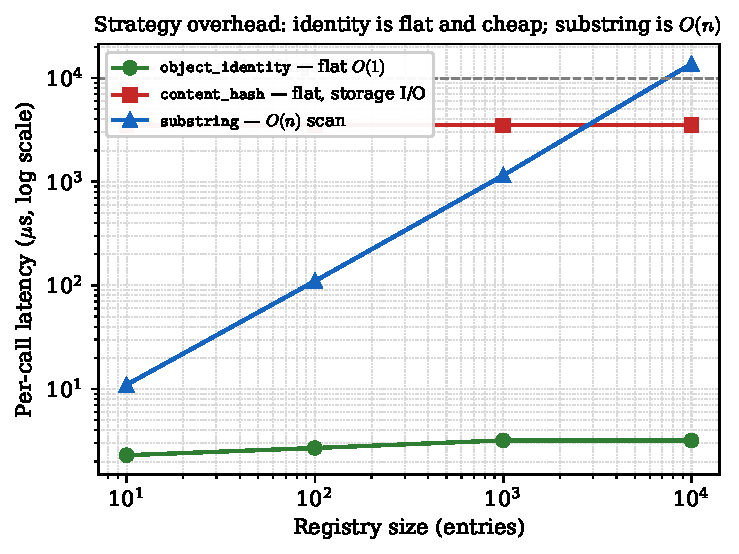
\includegraphics[width=0.72\linewidth]{figs/overhead.pdf}
\caption{Per-strategy instrumentation overhead vs.\ registry size (log--log; environment-specific
absolutes, portable shapes). \texttt{object\_identity} is flat $O(1)$ and effectively free;
\texttt{content\_hash} is flat but $\approx$1000$\times$ costlier (storage I/O); \texttt{substring} grows
$O(n)$ and crosses the cost of a typical ${\sim}10$\,ms embeddings call near $10^4$ entries. Because the
linker is first-match-wins, the expensive strategies run only on an object-identity miss, so the common
path is dominated by the flat green curve.}
\label{fig:overhead}
\end{figure}

Because the strategies are first-match-wins, the expensive ones run \textbf{only on object-identity miss}.
The \textbf{common-path} end-to-end cost (register + correlate, identity hit) is \textbf{9.5\us $\approx$
0.095\% of a ${\sim}10$\,ms embeddings call (0.0019\% of a ${\sim}500$\,ms chat call)}. The two fallback
costs are \emph{characterized and mitigable}: content-hash's per-query storage I/O can be batched/deferred;
substring's $O(n)$ scan is an inverted-index roadmap item (the strategy to watch as the registry approaches
its cap). Accuracy says the linker is \emph{correct}; overhead says it is \emph{affordable in the common
case, with bounded fallback costs}.

\subsection{The trust-envelope map (the applied payoff)}

Because the FP mechanisms concentrate in the lower confidence bands, \textbf{a confidence threshold is a
precision/recall knob with known content.} This table is from the \textbf{same $N=900$ corpus} as
\S5.1--5.4; its \emph{Precision} \textbf{and} \emph{Recall} are both \textbf{cumulative}, computed over all links
(resp.\ all positives) at confidence $\geq$ the threshold, a different cut from \S5.1's \emph{per-band}
precision and \S5.2's \emph{per-mechanism} recall. So both columns differ from those sections by
construction, not by inconsistency: the cumulative $\geq$0.80 precision (0.941) versus the per-band 0.80
precision (0.800); and the cumulative $\geq$1.00 recall (0.160 $=$ verbatim's 100 correct of all 625
positives) versus verbatim's per-mechanism recall (1.000 $=$ 100 of 100 verbatim positives). Different
denominators, distinct quantities.

\begin{table}[h]
\centering
\small
\begin{tabular}{@{}llll@{}}
\toprule
Threshold & Precision (cumulative) & Recall (cumulative) & Admits FP modes \\
\midrule
conf $\geq$ 1.00 & 1.000 [0.96, 1.00] & 0.160 [0.13, 0.19] & (none) \\
conf $\geq$ 0.95 & 1.000 [0.99, 1.00] & 0.480 [0.44, 0.52] & (none) \\
conf $\geq$ 0.80 & 0.941 [0.91, 0.96] & 0.640 [0.60, 0.68] & hash-aliasing \\
conf $\geq$ 0.70 & 0.909 [0.88, 0.93] & 0.800 [0.77, 0.83] & hash-aliasing, substring-collision \\
\bottomrule
\end{tabular}
\end{table}

\begin{itemize}[leftmargin=*]
\item \textbf{FP-intolerant deployments (audit/regulated): threshold at confidence $\geq$ 0.95} $\rightarrow$
precision 1.000 (95\% CI [0.99, 1.00]), excluding \emph{both} characterized FP modes.
\item \textbf{Recall-maximizing deployments: $\geq$ 0.70} $\rightarrow$ recall 0.800, admitting the two (now
named) FP modes.
\item \textbf{Structural blind spot at any threshold:} paraphrased-derived links are unrecoverable until
\texttt{name\_match} is implemented.
\end{itemize}

The \textbf{threshold\dto{}FP-mode mapping} (which modes appear at which threshold) is
\textbf{composition-robust}: fixed by which confidence band each mechanism occupies, and unchanged from
the smaller pilot run; only the values shift. The \emph{recall values} remain composition-dependent (they
track the positive/negative mix) and are read as on-corpus, not as portable rates.

\section{Threats to Validity}

Pre-registered and restated honestly:
\begin{itemize}[leftmargin=*]
\item \textbf{T1: constructing the test to flatter the system.} Mitigated by Arm C (adversarial, by
design) and by reporting per-arm; we refuse a single blended headline figure.
\item \textbf{T2: ground-truth annotation error (Arm B).} A frozen annotation guide, two blind
annotators, $\kappa$ reported, third-party adjudication; pre-committed $\kappa$ thresholds and the response
to missing them.
\item \textbf{T3: self-authored pipelines.} Arm B requires $\geq$2 third-party pipelines we did not
write.
\item \textbf{Small per-band $N$ / composition-dependent values.} The per-band precision \emph{values} for
inferred strategies are corpus-composition-dependent; only the monotonic structure, object-identity
precision, per-mechanism recall, and the representative FPR are quotable as bare linker properties (\S5.1).
\item \textbf{Synthetic-only ecological validity.} The headline accuracy is established on constructed
pipelines; real-pipeline validation is in progress and is required before the inferred-strategy precision
\emph{values} are claimed for real workloads.
\item \textbf{Single-environment overhead.} Absolute latencies are environment-specific; the ratios
(content-hash $\approx$1000$\times$ identity) and shapes (identity flat, substring $O(n)$) are portable.
\end{itemize}
Stating these \emph{is} the credibility: an evaluation that reports 1.0 everywhere with no stated limits
invites the suspicion it earns.

\section{Discussion: Deployment Guidance}

The trust-envelope map (\S5.7) converts the calibration finding into an operational knob. A deployer chooses
a confidence threshold knowing \emph{exactly} which failure modes each setting admits: an FP-intolerant
audit deployment thresholds at $\geq$0.95 and accepts reduced recall; a recall-maximizing deployment accepts
the two named, bounded FP modes. The overhead profile (\S5.6) supports leaving instrumentation \textbf{on in
production}: the common path costs $<0.1\%$ of an LLM call, and the two fallback costs are mitigable by
batching (content-hash) and indexing (substring). Together these empirically back leaving instrumentation
\textbf{always-on} for the path that dominates, with its costs and limits named rather than hidden. (The
\emph{zero-egress} property, meaning the linker runs in-process and no data leaves the host, is
\textbf{architectural}, not a result of this study; we note it as deployment context, not as something
measured here.)

\section{Limitations and Future Work}
\begin{itemize}[leftmargin=*]
\item \textbf{Ecological validity (Arm B).} The benchmark's most important next step: $\geq$2 annotated
third-party pipelines to (a) supply the representative input distribution that turns the inferred-strategy
precision \emph{values} into real numbers, and (b) furnish the pre-emption \emph{correctness} evidence
currently absent by design (\S5.5). Arm B slots into a proven scoring contract.
\item \textbf{Substring scaling.} $O(n)$ registry scan (13.75\,ms at $10^4$ entries); an inverted index
would flatten it.
\item \textbf{Recall ceiling.} Paraphrased/derived links are unrecoverable until the \texttt{name\_match}
strategy ships; this is a roadmap item, not a bug.
\item \textbf{One link per call (multi-parent provenance).} The linker emits a single best link per LLM
call, so for a call whose input genuinely derives from \emph{multiple} upstream artifacts (e.g.\ a RAG
prompt assembled from several retrieved chunks) it recovers \emph{a} correct parent but not the
\emph{complete} parent set. We report \textbf{link-level recall} (did it find a correct parent?) as the
headline; \textbf{provenance-completeness} (the fraction of all true parents recovered) is structurally
capped for multi-parent calls and is the natural target of a future multi-link mode.
\item \textbf{Causal root-cause analysis} over the recovered lineage is a v1.0+ track beyond this paper's
accuracy scope.
\end{itemize}

\section{Conclusion}

We measured a cross-domain data\dto{}LLM lineage linker with a construction-based benchmark that makes ground
truth tractable and an adversarial arm that makes failure measurable. The linker's confidence scale is
calibrated in structure; its exact-match strategy is near-perfectly precise; it shows no observed false
positives on representative new data; its false-positive surface is two bounded, characterized mechanisms;
and its common-path overhead is below 0.1\% of an LLM call. The result is not a claim of perfection but a
\textbf{map of when the linker should and should not be trusted}, which, for an audit tool, is the more
useful and the more credible contribution. Real-pipeline ecological validation is the next step.

\section*{Reproducibility}

Methodology and all decisions, including the pre-registration and the dated implementation-resolved
refinements of \S4.4, are recorded in the project's methodology log. Corpus generators, the scoring
harness, the overhead harness, and the trust-map analysis are released as code at
\url{https://github.com/kishanraj41/rudriq}, under \texttt{paper2/}. The scored $N=900$ corpus that
every figure in \S5.1--5.5 is drawn from is serialized to \texttt{scale\_up\_n900.json} (under
\texttt{paper2/corpus/artifacts/}), regenerated by \texttt{python -m paper2.corpus.scale\_up}; the
\S5.7 threshold sweep is serialized to \texttt{trust\_map.json}. Smaller per-arm verification corpora
ship alongside them for the construction-consistency gate (\S4.3). Accuracy results are deterministic
and re-run against the real linker; overhead figures are distributional and environment-specific (\S5.6).

\bibliographystyle{plainnat}
\bibliography{refs}

\end{document}
